\scanpage{142}
% lines 1–5
$f:X\to S$ projectif et lisse, fibres géom connexes de dim 1.

$U=X-Y$, \inserted{$Y$ sous-schéma fermé de $X$ \uline{étale} sur $S$} \deleted{\unsure{$Y$}} [\inserted{p. ex. $Y=$} $\coprod_{i\in I}g_i(S)$, les $g_i$ des sections telles que les $g_i(S)$ deux à deux disjoints]

$f_U:U-S$

$n$ premier aux car. résiduelles \inserted{de $S$}. On trouve
\[
E^{pq}_{2}=H^p(S,\underbrace{R^q_{!}f_U(\mu_n)}_{\substack{0\ \text{sauf si}\\q=1,2}})\Longrightarrow H^{*}_{\mathrm{prop}}(\deleted{\unsure{X}}U,\mu_n)
\]
% lines 6–9
\[
R^q_{!}f_U(\mu_n)=
\begin{cases}
0 & \text{si }q\deleted{\ne}\inserted{\notin}\{1,2\\
{}_{n}E & \text{si }q=1\qquad\text{(cf plus bas \inserted{déf. de $E$})}\\
(Z/nZ)_S & \text{si }q=2
\end{cases}
\]
\figure{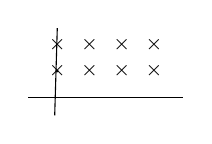
\begin{tikzpicture}[x=.41cm,y=.33cm]
\draw (-.9,0)--(3.9,0); \draw (-.08,-.7)--(0,2.65);
\foreach \x in {0,1,2,3}{\foreach \y in {1,2}{\node at (\x,\y) {\scriptsize $\times$};}}
\fill (0,1) circle (.05);
\end{tikzpicture}}
\diagram{\begin{tikzcd}[ampersand replacement=\&,row sep=small]
E_2^{02}\arrow[r]\arrow[d,equal] \& E_2^{2,1}\arrow[d,equal]\\
H^0(S,Z/nZ) \& H^2(S,{}_{n}E)
\end{tikzcd}}

% lines 10–14
On trouve un élément canonique
\[
\xi_n\in H^2(S,{}_{n}E)
\]
Si $n=l^{\unsure{\nu|v}}$ ($\nu$ variable), $l$ premier distinct des car. rés. sur $S$, on trouve
\[
\boxed{\xi(l)\in H^2(S,T_l(E))}
\]
Cet \uline{élément est nul si} $U$ a \uline{une section sur} $S$.

% lines 15–18
$E$ est un schéma en groupes lisse sur $S$, \deleted{\unsure{tel}} \inserted{à fibres connexes,} extension de $J=\underline{\mathrm{Pic}}^{0}_{X/S}$ par $T=G_m^{I}/\underset{\longrightarrow\,\text{diagonale}}{G_m}$,
\diagram{\begin{tikzcd}[ampersand replacement=\&,row sep=small]
0\arrow[r] \& T\arrow[r]\arrow[d,equal] \& E\arrow[r] \& J\arrow[r] \& 0\\
{} \& G_{m_S}^{I}/G_{m_S} \& {} \& {} \& {}
\end{tikzcd}}
% archive sheet number: 141

